%!TEX root = ../main.tex
\section{Data}
\label{sec:data}
In the data section, we describe the source of our data and how the factor strategies are constructed. We then present summary statistics including tests for autocorrelation and volatility clustering, as well as quantile-quantile (QQ) plots. Finally, we discuss the unconditional correlations of the factor strategies.

\subsection{Data description}

We use US data on factor strategies 1963--2016, which we download from Kenneth French's data library.\footnote{Kenneth French Data Library. (2016). \textit{Fama/French 5 Factors (2x3) [Daily]} and \textit{Momentum Factor (Mom) [Daily]}. Available from: \url{http://mba.tuck.dartmouth.edu/pages/faculty/ken.french/data_library.html}} We merge the daily Fama-French five-factor data set with the daily momentum data set. Both are available since 1963-07-01, making 1963-07-05 the first week of data. In our sample, 2016-07-01 is the last data point. 

While the related papers \textcite{FF2015} and \textcite{Asness2015} both use monthly data, we choose the weekly frequency for two main reasons: (1) We take a portfolio perspective rather than an asset pricing perspective, and believe that a more frequent horizon than monthly data is relevant for both rebalancing and risk management objectives, and (2) Due to computational limitations, the copula methodology discourages us from going to the daily frequency, as optimizations become significantly more time-consuming.

We proceed with descriptions of how factors are constructed. The Mkt.RF factor is long the value-weighted return of CRSP firms on NYSE, AMEX or NASDAQ with CRSP share codes 10 or 11 and short the one-month Treasury bill rate. The remaining return series are based on zero-cost portfolios that are long certain equities and short other equities, according to a 2 x 3 sort: First, firms are sorted into one of two size groups, small and big, depending on whether the market cap is above or below the median. In the small and big firm groups, each factor then sorts into one of three groups depending on whether the variable of interest falls below the 30\textsuperscript{th} percentile, between the 30\textsuperscript{th} and the 70\textsuperscript{th} or above the 70\textsuperscript{th}. For the six-factor data set, the remaining five factors are:
\begin{itemize}
  \item High-minus-low, is long firms above the 70\textsuperscript{th} percentile book-to-market and short stocks below the 30\textsuperscript{th} percentile, in the small and big firm group respectively.
  \item Conservative-minus-aggressive, is long firms above the 70\textsuperscript{th} percentile total asset growth and short firms below the 30\textsuperscript{th} percentile. 
  \item Robust-minus-weak, is long firms above the 70\textsuperscript{th} percentile operating profitability and short firms below the 30\textsuperscript{th} percentile. 
  \item Small-minus-big, is long firms below the 50\textsuperscript{th} percentile market cap and short firms above the 50\textsuperscript{th} percentile, in each of the three groups HML, CMA and RMW.
  \item Momentum, is long firms above the 70\textsuperscript{th} percentile prior 2-12 month return (i.e. excluding the last month) and short stocks below the 30\textsuperscript{th} percentile, in the small and big firm group respectively.
\end{itemize}
The sort ensures that SMB includes firms small and big firms equally from the remaining factors, and that the other factors include equal amounts of small and big firms. Note that momentum originates from a different data set and does not affect the SMB composition. French's financial statement data originates from Compustat, stock return data is from CRSP and Treasury return data is from Ibbotson Associates.

\subsection{Summary statistics}

%!TEX root = ../../main.tex

\begin{table}[ht!]
  \centering
  \footnotesize
  \renewcommand{\arraystretch}{1.2}

  \caption{Summary Statistics of Weekly Factor Returns}

  \begin{longcaption}
    \emph{Kurtosis} is excess kurtosis. \emph{LB} is the weighted Ljung-Box test up to 5 and 10 lags respectively, where the null hypothesis is no serial correlation~\autocite{FisherGallagher2012}. Data from 1963-07-05 to 2016-07-01 (2766 weeks).
  \end{longcaption}

  \label{tab:summarydata}

  \begin{tabularx}{\textwidth}{@{} l X dXdXdXdXdXd @{}}
    \toprule
      && \multicolumn{1}{c}{Mkt.RF}
      && \multicolumn{1}{c}{SMB}
      && \multicolumn{1}{c}{HML}
      && \multicolumn{1}{c}{CMA}
      && \multicolumn{1}{c}{RMW}
      && \multicolumn{1}{c}{Mom} \\
    \midrule
    Mean (\%)              & & 0.12   & & 0.04  & & 0.08  & & 0.07  & & 0.06  & & 0.16   \\
    % Annual                 & & 6.02   & & 2.19  & & 4.33  & & 3.78  & & 3.21  & & 8.18   \\
    SD (\%)                & & 0.27   & & 0.06  & & 0.05  & & 0.04  & & 0.05  & & 0.23   \\
    % Annual SD (\%)         & & 15.77  & & 8.76  & & 8.87  & & 6.37  & & 6.31  & & 13.24  \\
    Maximum (\%)           & & 13.46  & & 6.13  & & 12.46 & & 5.53  & & 9.87  & & 12.79  \\
    Minimum (\%)           & & -18.00 & & -9.34 & & -7.93 & & -4.28 & & -5.99 & & -16.04  \\
    Median (\%)            & & 0.27   & & 0.06  & & 0.05  & & 0.04  & & 0.05  & & 0.23   \\
    Skewness               & & -0.44  & & -0.38 & & 0.50  & & 0.37  & & 0.92  & & -1.07  \\
    Kurtosis               & & 5.27   & & 4.50  & & 7.95  & & 3.24  & & 14.18 & & 10.19   \\
    \midrule
    \multicolumn{8}{@{}l}{\textbf{p-values of Ljung-Box (LB) tests on Returns and Squared Returns}} \\
    Returns LB(5)          & & 0.26   & & 0.00  & & 0.00  & & 0.00  & & 0.00  & & 0.00   \\
    Returns LB(10)         & & 0.00   & & 0.00  & & 0.00  & & 0.00  & & 0.00  & & 0.00   \\
    Squared Returns LB(5)  & & 0.00   & & 0.00  & & 0.00  & & 0.00  & & 0.00  & & 0.00   \\
    Squared Returns LB(10) & & 0.00   & & 0.00  & & 0.00  & & 0.00  & & 0.00  & & 0.00   \\
    \midrule
    \textbf{Correlations}
      && \multicolumn{1}{c}{Mkt.RF}
      && \multicolumn{1}{c}{SMB}
      && \multicolumn{1}{c}{HML}
      && \multicolumn{1}{c}{CMA}
      && \multicolumn{1}{c}{RMW}
      && \multicolumn{1}{c}{Mom} \\
    \midrule
    Mkt.RF && 1.00  &&       &&       &&       &&      && \\
    SMB    && 0.08  && 1.00  &&       &&       &&      && \\
    HML    && -0.28 && -0.03 && 1.00  &&       &&      && \\
    CMA    && -0.42 && -0.05 && 0.63  && 1.00  &&      && \\
    RMW    && -0.15 && -0.34 && -0.05 && -0.06 && 1.00 && \\
    Mom    && -0.12 && -0.01 && -0.22 && 0.07  && 0.08 && 1.00 \\
    \bottomrule
  \end{tabularx}
\end{table}


For all factors, there are 2,766 consecutive data points and no missing data. Mkt.RF is the most volatile and extreme of the series, with weekly returns between -19.8\% and 12.6\% and a weekly volatility of 2.2\%. CMA and RMW seem to be less extreme than HML, with less negative minimums and smaller volatilities. The factor strategies have excess kurtosis, or fat tails, which is typical for financial returns. The excess kurtoses of the Mom, HML and RMW factors are even higher than the kurtosis of the Mkt.RF factor, where RMW is exceptionally high at 13.0. However, while market returns are negatively skewed, HML, CMA and RMW instead exhibit positive skewness. QQ-plots versus normal theoretical quantiles in \autoref{fig:qq_returns} graphically show the non-normality.

\begin{figure}[ht!]
  \centering
  \footnotesize
  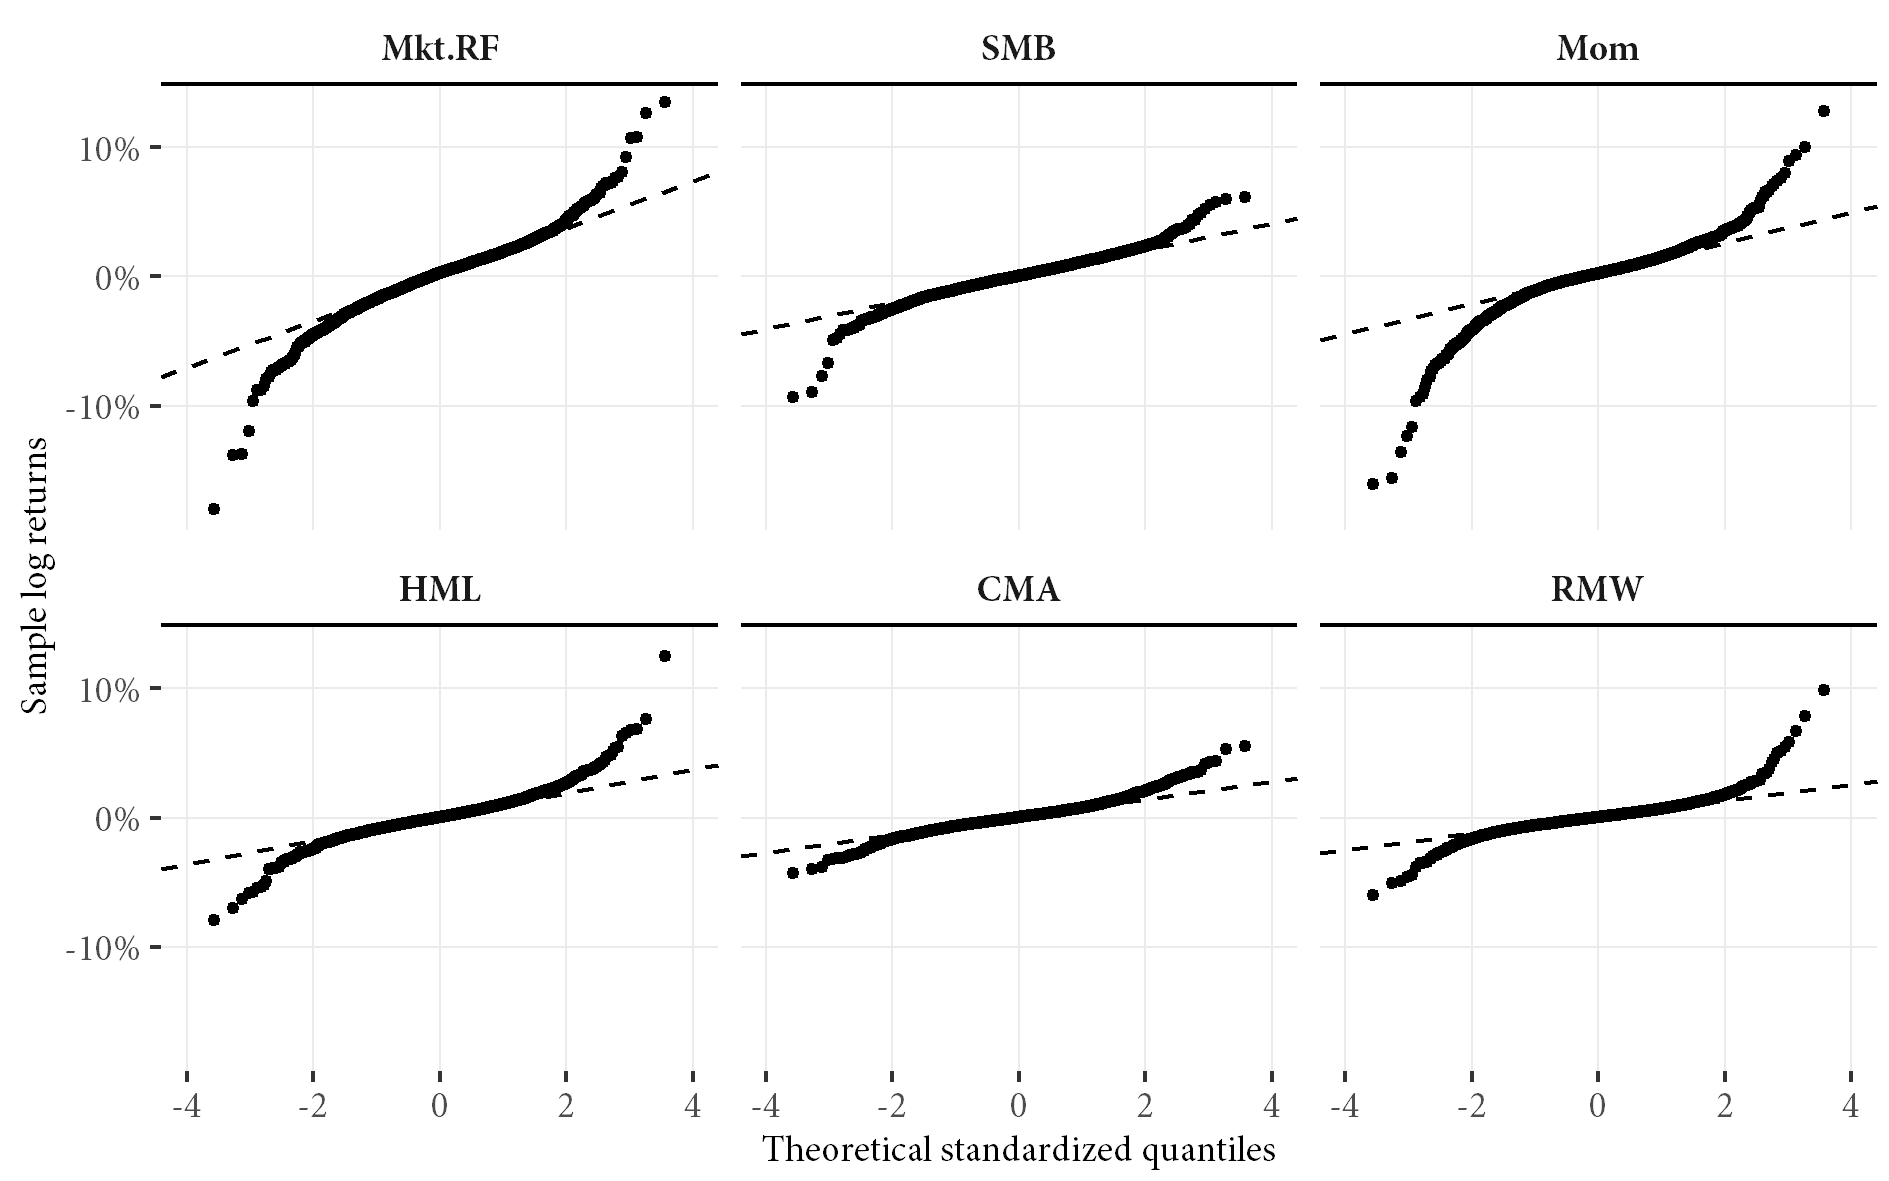
\includegraphics[scale=1]{graphics/qq_returns.png}
  \caption{QQ-plots of return series}
  \begin{longcaption}
    Data from a normal distribution should line up on the dashed line. Based on weekly returns 1963--2016.
  \end{longcaption}
  \label{fig:qq_returns}
\end{figure}

We conduct Ljung-Box tests of the factor returns to control for weekly autocorrelation.\footnote{For a detailed description of the test, see \autoref{app:univariate_diagnostics}.} The p-values of these tests are given in \autoref{tab:summarydata} and are very low for all factors except Mkt.RF, leading to a strong rejection of the zero autocorrelation null hypothesis. For Mkt.RF, the p-value is not small enough for a rejection of zero autocorrelation at the 5 week maximum lag length, but strongly rejected at the 10 week maximum lag length. We also conduct Ljung-Box tests of the squared factor returns to control for volatility clustering (ARCH effects). Here, the null hypothesis is that there are no ARCH effects, and p-values given in \autoref{tab:summarydata} strongly reject the null for all factors, both at max lag length of 5 and 10 weeks.\footnote{The lag lengths were chosen after visual inspection of autocorrelation function  plots.}

We conclude that factor return series are non-normal and that returns are not independently distributed over time -- more specifically, past returns have predictive power on future returns, and past volatility has predictive power on future volatility, i.e. the series exhibit both autocorrelation as well as autoregressive heteroscedasticity. These predictable phenomena in financial return data are typically captured by models that incorporate autoregressive components for both the conditional mean and variance equations, such as the family of ARMA-GARCH models, which is further discussed in \autoref{sec:modeling_of_factor_returns}.
\begin{figure}[htbp]
  \centering
  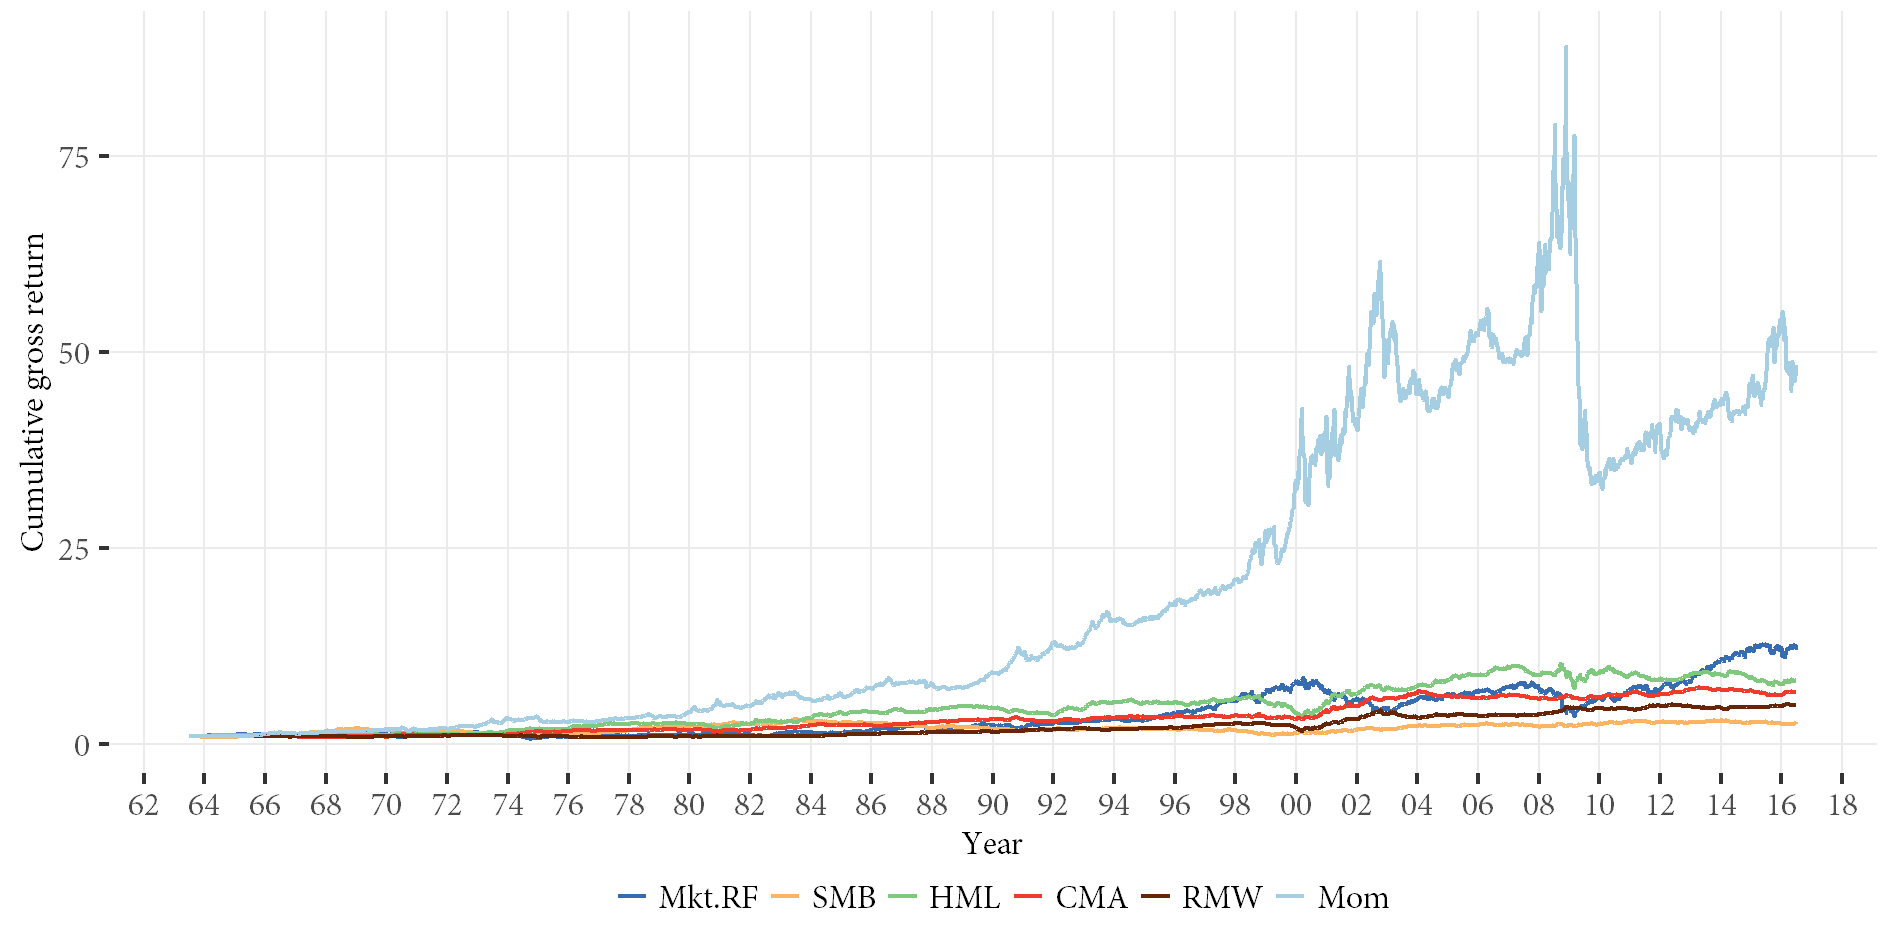
\includegraphics[scale=1]{graphics/cumretPlot.png}  
  \footnotesize
  \caption{Cumulative returns to factor strategies}
  \begin{longcaption}
    Cumulative returns to investing one dollar in each factor strategy, beginning 1963-07-05. Based on weekly returns 1963--2016.
  \end{longcaption}
  \label{fig:cumret}
\end{figure}
\begin{figure}[htbp]
  \centering
  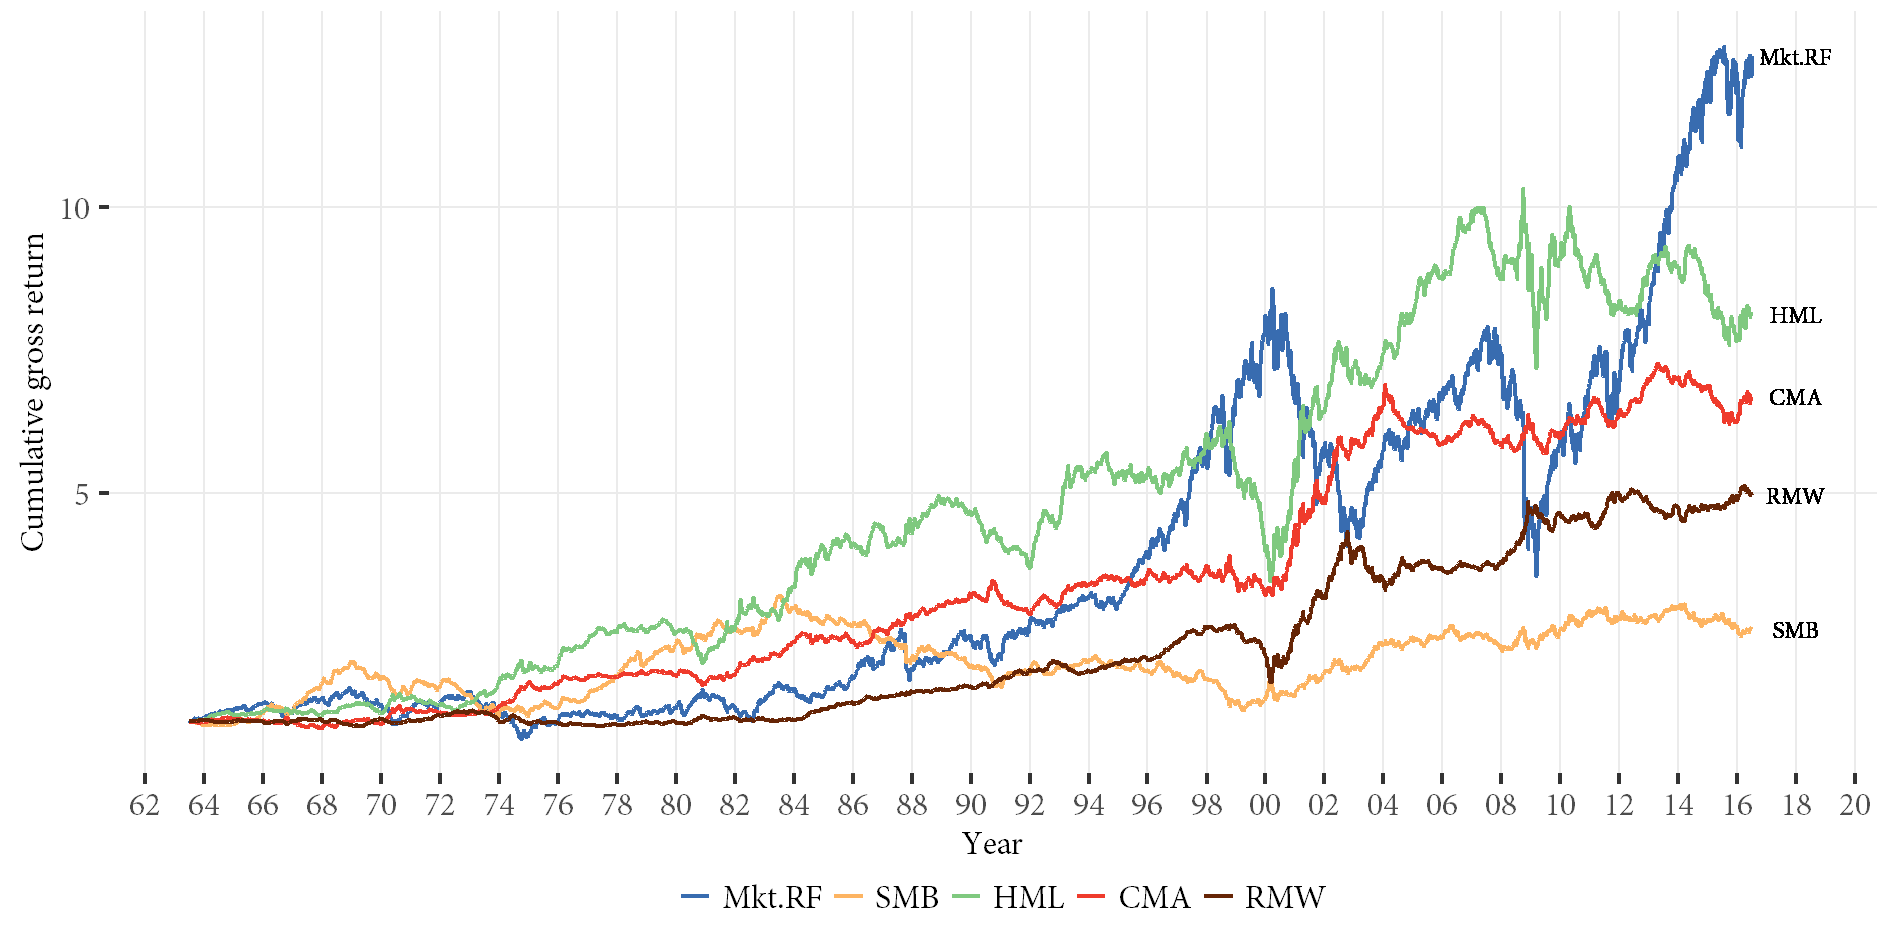
\includegraphics[scale=1]{graphics/cumretPlot_no_mom.png}  
  \footnotesize
  \caption{Cumulative returns to factor strategies, excl. momentum}
  \begin{longcaption}
    Cumulative returns to investing one dollar in each factor strategy, beginning 1963-07-05. Based on weekly returns 1963--2016.
  \end{longcaption}
  \label{fig:cumret_no_mom}
\end{figure}
\begin{figure}[htbp]
  \centering
  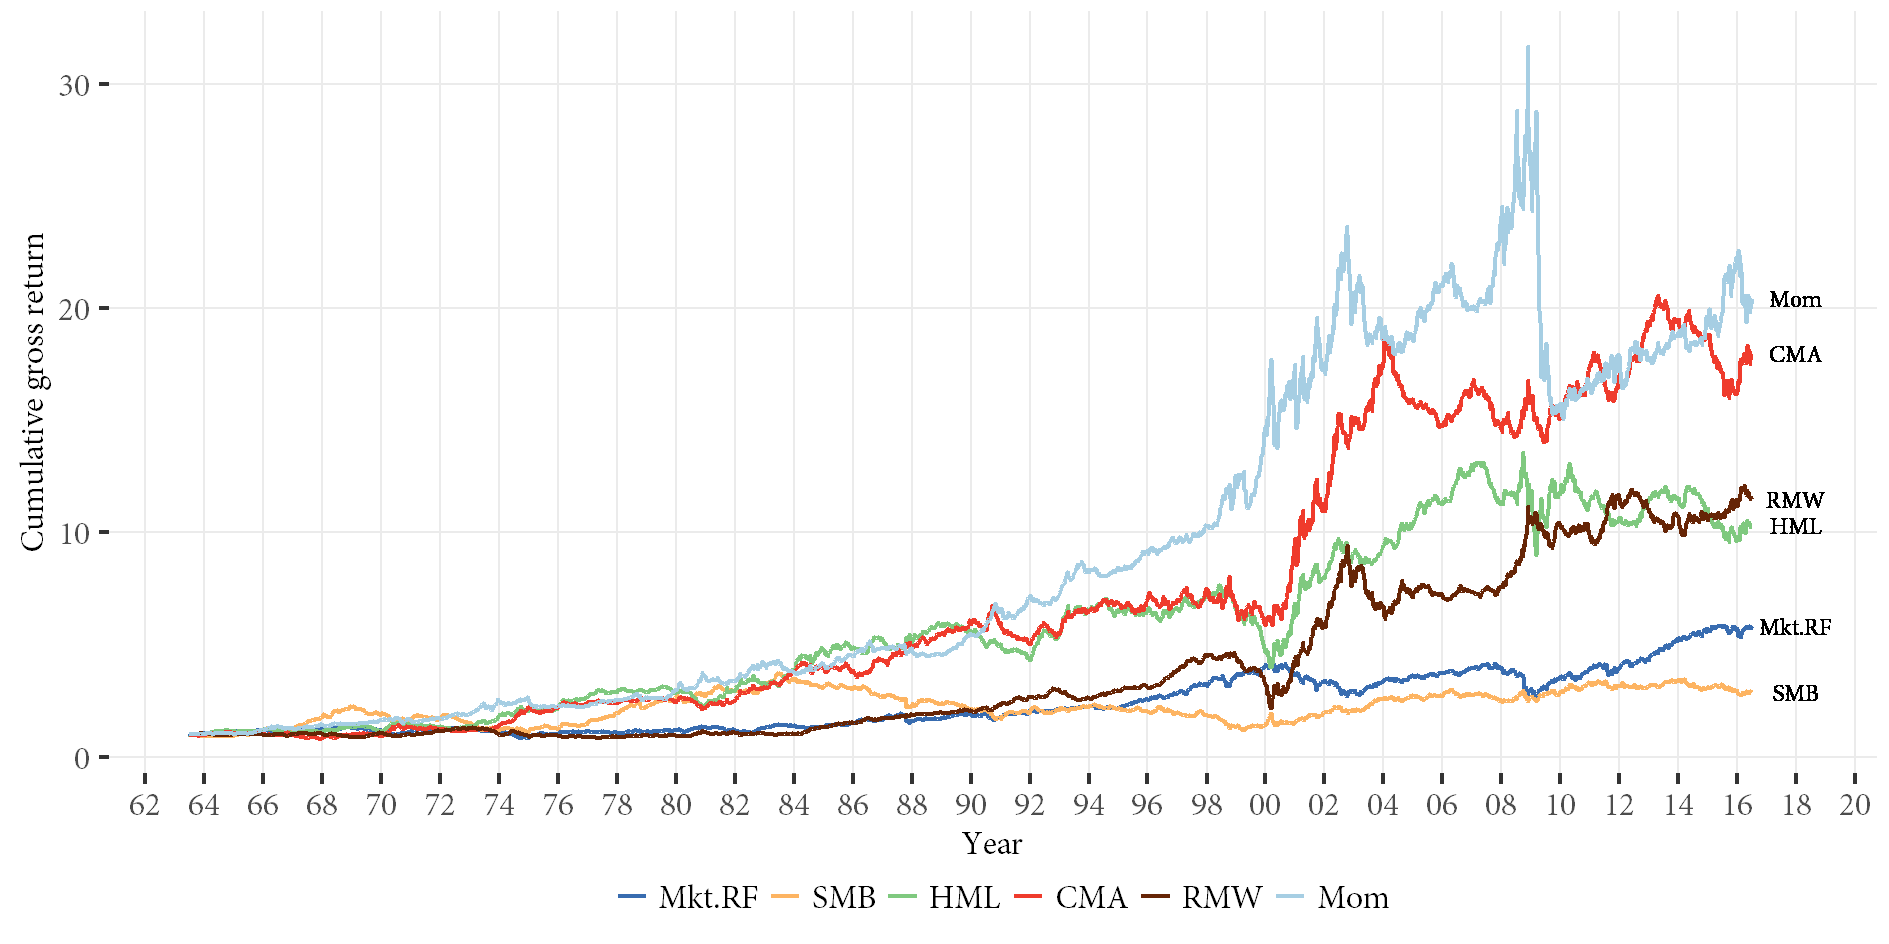
\includegraphics[scale=1]{graphics/cumretStdPlot.png}  
  \footnotesize
  \caption{Standardized cumulative returns to factor strategies}
  \begin{longcaption}
    Cumulative returns to investing one dollar in each factor strategy, standardized to 10\% annual volatility, beginning 1963-07-05. Based on weekly returns 1963--2016.
  \end{longcaption}
  \label{fig:cumretstd}
\end{figure}

A plot of cumulative gross returns (\autoref{fig:cumret}) clearly show the high returns to the momentum strategy throughout the sample period. Taking out momentum, \autoref{fig:cumret_no_mom} shows that the Mkt.RF factor has the second highest cumulative gross return, but also that it is the most volatile of the remaining strategies. We normalize the series to 10\% annual volatility in \autoref{fig:cumretstd}, which gives a more nuanced picture of risk-adjusted performance. Since 1963, each of the strategies except for SMB has outperformed the market factor. Furthermore, factor strategies seem to crash at different times and diversify each other (e.g. Mom performed well during the bubble of 1999--2000 and RMW performed well during the recession of 2007--2009).

Looking at the correlation matrix of factor returns, the generally low or even negative correlation coefficients indicate the diversification benefits of factor strategies. The HML--CMA pair does stand out, however, with an unconditional correlation of 0.63, which could be related to a partial overlap of the factor components, as discussed in \autoref{sec:literature} -- past investment is shown to be negatively empirically related to the current book-to-market ratio. The substantially higher correlation in this asset pair indicates smaller diversification benefits. We also note that the new factor RMW has an interesting pattern of low of negative correlations to all other factors, which indicates diversification benefits.
\FloatBarrier

